\documentclass[conference]{IEEEtran}
\IEEEoverridecommandlockouts
\usepackage{cite}
\usepackage{amsmath,amssymb,amsfonts}
\usepackage{algorithmic}
\usepackage{graphicx}
\usepackage{textcomp}
\usepackage{xcolor}
\def\BibTeX{{\rm B\kern-.05em{\sc i\kern-.025em b}\kern-.08em
    T\kern-.1667em\lower.7ex\hbox{E}\kern-.125emX}}
\begin{document}

\title{Exploring Fairness Constraints on Models of German Credit Risk}

\author{\IEEEauthorblockN{FSDN71}
\IEEEauthorblockA{\textit{Department of Computer Science} \\
\textit{University of Durham}\\
Durham, United Kingdom \\
fsdn71@durham.ac.uk}
}

\maketitle

\begin{abstract}
    Allocation of credit, a fundamental component of the economy, has direct and lasting impacts on the prosperity of lenders, borrowers, and the wider population. Models which utilise machine learning techniques in order to aid in credit decision-making often need to select a trade-off between accuracy and bias, due to the different distributions of characteristics among members of different legally protected classes such as gender. This report documents a project of analysis, prediction and reproduction of fairness-enhancing methods on machine learning models to predict credit risk scores.
\end{abstract}
\section{Project Proposal}
Credit risk prediction is a highly valuable problem with measurable effects on real-world financial security. Given a set of characteristics of one person, a predictor must estimate whether the person would be likely to default on a loan, in order to decide whether to grant or deny such a loan. However, due to historical biases both inside and outside of financial institutions, demographics such as gender often show disparities, both in error and in outcome. This report proposes to analyse and measure prediction performance of machine learning models with and without the application of fairness constraints.
\subsection{Motivation}
Credit is a core pillar of the wider economy, enabling efficient distribution of funds in order to maximise value. This broadly falls into two main categories - lending to corporations, and lending to individuals. There has been a high volume of research into modelling corporate bankruptcy risk\cite{article}\cite{provenzano2020machine}, as well as individual loan default rates\cite{gcr}. The importance of accuracy in predicting loan defaults has increased considerably after events such as the Financial Crisis of 2008, in which a consistent failure to appropriately model and incorporate default risk into loan-granting decision processes resulted in the widespread financial catastrophe.

However, there also exists the question of bias in such predictive models. Research has found that algorithms predicting loan default rates often retain or exacerbate existing disparities across protected characteristic groups such as gender or ethnicity\cite{bias}. This raises several questions of appropriate decision-making capabilities for algorithms- whether it is possible or desirable for algorithms to be constrained in their predicted outputs in order to equalise or rectify existing biases.
\subsection{Dataset}
The dataset that will be used in this project is the German Credit Risk dataset. This contains a combination of qualitative and quantitative variables such as category of requested credit purpose and installment rate as a percentage of disposable income - information that is highly informative in predicting default risk. The dataset also contains information on three protected classes, only two of which have previous research on mitigating algorithmic bias - age and sex. The third is marital status, which is a protected class in the United Kingdom and in the United States, however the this is unlikely to be usable, due to the fact that the female-unmarried label does not appear in the dataset.
\subsection{Implementation}
The implementation of the proposed project is guided by the approach shown in \cite{main} and will involve the following tasks:
\begin{enumerate}
    \item Dataset cleaning: transforming the original dataset into a form usable by most machine learning algorithms. This will use Python and packages such as Pandas and NumPy in order to filter and transform discrete variables, as well as partitioning into training, validation and testing sets.
    \item Dataset analysis: a data-informed explanation of any existing biases in the dataset in relation to any of the three protected classes identifiable, with quantitative descriptions of the direction and extent.
    \item Conventional machine learning application: using regular machine learning techniques, a predictor will be trained and evaluated using the partitioned datasets. Performance metrics, both in accuracy and bias, will be recorded for comparison.
    \item Evaluation of the conventional model re-trained and re-tested on an unbiased subsample of the dataset: an analysis of any differences in bias an accuracy.
    \item Implementation of a fair machine learning method - in this case, the Geometric Repair approach outlined in \cite{main}, in order to debias the dataset.
    \item Evaluation of fairness improvements and conclusions of use-cases.
\end{enumerate}

The final outcome of the project will be an analysis of the original dataset, and the bias-accuracy tradeoff present in the application of the fairness method. 
\section{Project Progress}
\subsection{Data Analysis}
\paragraph{Adjustments} The dataset\footnote{Available at https://archive.ics.uci.edu/ml} required a number of adjustments:
\begin{enumerate}
    \item Decoding categorical codes into descriptive names for visualisation purposes
    \item Encoding of categorical features into one-hot form: this applied to columns describing credit history, savings account ownership, property ownership, job and employment status.
    \item Extraction of gender, as well as binning of age ($Age >= 25$).
    \item No continuous feature normalisation is applied in order to be comparable to the fairness methods to be used.
\end{enumerate}
\paragraph{Demographic breakdowns} The dataset was broken down by age category and gender - four distinct groups. In the implementation notebook are four tables, each containing the mean and variance for each continuous column, as well as the top 3 values for each categorical column (where at least 3 distinct values exist). There are a number of interesting observations: firstly, that there is a bias in the amount requested to borrow by gender - men typically borrow higher amounts. The quantiles of amounts borrowed for each age-gender breakdown are shown in Figure \ref{fig:quantiles}.
\begin{figure}[h]
    \centering
    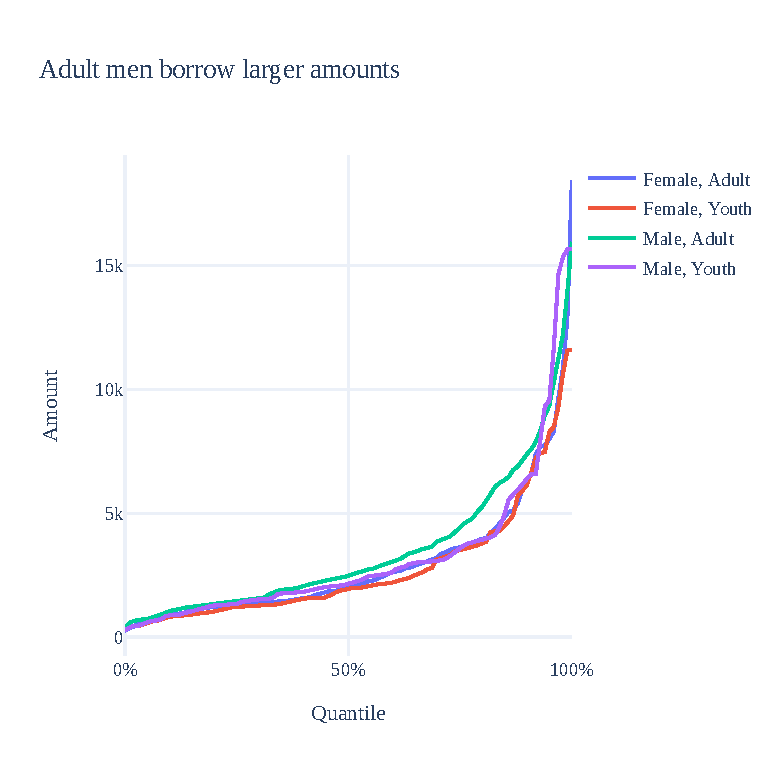
\includegraphics[width=0.5\textwidth]{../implementation/images/borrow_quantiles.pdf}
    \caption{Quantiles for amount borrowed, for each protected class}
    \label{fig:quantiles}
\end{figure}
Furthermore, the distribution of credit history categories varies by age-gender subgroup. Figure \ref{fig:credit_cat} shows the distribution for each subgroup - older applicants, especially men, are more likely to have disadvantageous credit histories. While there is not a clear trend, it is clear that the disparity is large enough in each category for the protected subgroup to be partially predictable.
\begin{figure}[h]
    \centering
    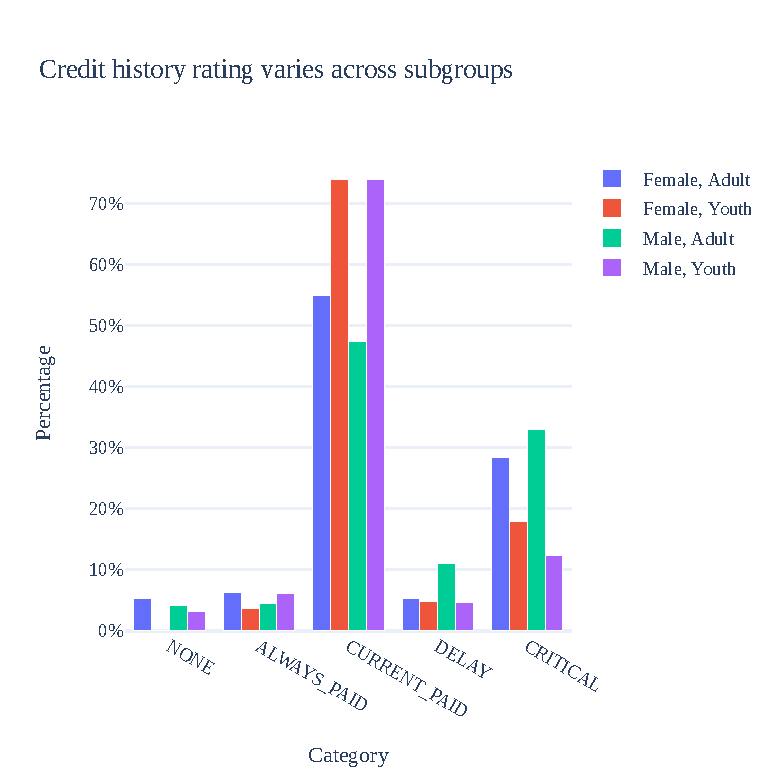
\includegraphics[width=0.5\textwidth]{../implementation/images/credit_ratings.pdf}
    \caption{Distribution of credit category frequencies per subgroup}
    \label{fig:credit_cat}
\end{figure}
\bibliographystyle{IEEEtran}
\bibliography{project_proposal}

\end{document}
